\documentclass[a4paper]{article}
\usepackage{graphicx} %Required for diagrams
\usepackage[bookmarks=true]{hyperref}
\usepackage{bookmark}%Required to do pdf bookmarking
\usepackage[margin=1.2in]{geometry}
\usepackage{float}
\usepackage{caption}
\usepackage{hyperref}%Required for referencing website pages
\usepackage[english]{babel}

\usepackage{graphicx}
\usepackage{dcolumn}
\usepackage[table]{xcolor}

\title{User Manual}
\author{Baobab Team}

\begin{document}
\newpage

\begin{titlepage}

\begin{center}


\includegraphics[width=400px]{pictures/logo.jpg}
\vspace{0.5 cm}
\begin{flushright} \large
\begin{tabular}{lr}
\vspace{1 cm}
\LARGE\textbf{Document:}Sprint Report 6\\

\vspace{1 cm}
\LARGE\textbf{Project:} Group Chat For Linphone (Agile DO-178)\\
\vspace{1 cm}
\LARGE\textbf{Advisor:} Kobus Coetzee\\
\vspace{1 cm}
\LARGE\textbf{Sponsors:} Nanoteq \& Department of Computer Science, UP\\
\vspace{1 cm}
\LARGE\textbf{Date: }\today\\
\end{tabular}
\end{flushright}

\centering 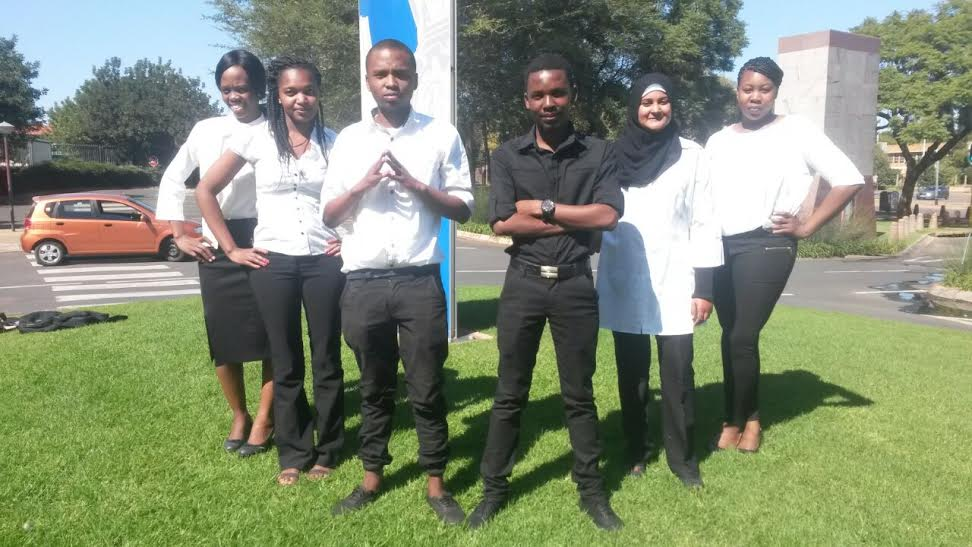
\includegraphics[width=350px]{pictures/Team.jpg}

Patience Mtsweni, Lerato Molokomme, Tsepo Ntsaba, Mpedi Mello, Lutfiyya Razak, Ephiphania Munava\\


\end{center}
\end{titlepage}
\newpage

\section{Introduction}
This user manual provides instructional support and guidance to help the users who use Linphone-android. The manual focuses on system configuration, installation, using the system, troubleshooting, etc.

\section{General Information}


\subsection{Project Details}

%Lerato edit here - System name and the names and/or affiliation of all stakeholders.
\setlength{\arrayrulewidth}{0.5mm}
\setlength{\tabcolsep}{12pt}
\renewcommand{\arraystretch}{2} 
\begin{tabular}{ |p{3cm}|p{3cm}|p{3cm}|  }
\hline
\rowcolor{lightgray}\multicolumn{2}{|c|}{Scrum User Roles} \\
\hline
Role & Name\\
\hline
Scrum master  & Potego Mello\\ \hline 
Client representative  & Patience Mtsweni\\ \hline 
UX developer  & Lutfiyya Razak and Lerato Molokomme\\ \hline 
Backend developer  & Ephiphania Munava and Potego Mello\\ \hline 
Crypto developer  & Tsepo Ntsaba \\ \hline 
CI / CD support  & Patience Mtsweni \\ 
\hline
\end{tabular}

\newpage
\subsection{System Overview}

\newpage
\subsection{System Configuration}
\\
The main aim of the functionality we are developing in the linphone project is to allow a group of users to be
able to communicate or exchange messages with each other. This functionality is achieved by creating a group
chat where there will be an interface that allows those messages to be exchanged and viewed. A  participant can
send messages and pictures to a group, send voice recordings,update the group picture and change the  group name.
A participant can become an administrator in the group -  usually this is the person who creates the group ,who is 
responsible for adding and  removing other participants.
\\
%Ephiphania Edit Here

\newpage
\subsection{Installation}
\begin{itemize}
\item Turn on your Android Smartphone and click on the Google Play icon to launch Google Play.
\item Tap the “Search” button in the upper right corner and type “Linphone”
\item From the result list tap the result with the title “Linphone Video” to expand it
\item Tap the “Install” button, Linphone for Android will be downloaded and the installation procedure will begin
\item Confirm that you accept the Linphone application rights on the screen that will be appear on your Smartphone by tapping “Accept”. When the file installation is done tap “Open”.
\item Press “Agree” when the License Agreement appears on your screen to finalize the install and start Linphone for Android.
\end{itemize}

\newpage
\subsection{Getting started}
%Patience Edit Here

\newpage
\subsection{Using the system}
%Potego Edit Here

\newpage
\subsection{System Configuration}
%Tsepo Edit Here
\newpage
\end{document}
